% ****** final-report.text ******
% ****** Start of file final-report.tex ******
%
%   This file is part of the APS files in the REVTeX 4.1 distribution.
%   Version 4.1r of REVTeX, August 2010
%
%   Copyright (c) 2009, 2010 The American Physical Society.
%
%   See the REVTeX 4 README file for restrictions and more information.
%
% TeX'ing this file requires that you have AMS-LaTeX 2.0 installed
% as well as the rest of the prerequisites for REVTeX 4.1
%
% See the REVTeX 4 README file
% It also requires running BibTeX. The commands are as follows:
%
%  1)  latex final-report.tex
%  2)  bibtex final-report
%  3)  latex final-report.tex
%  4)  latex final-report.tex
%
\documentclass[%
 reprint,
 amsmath,amssymb,
 aps,
 nofootinbib,
 showpacs
]{revtex4-1}

\usepackage{graphicx}% Include figure files
\usepackage{dcolumn}% Align table columns on decimal point
\usepackage{bm}% bold math
\begin{document}

\preprint{APS/123-QED}

\title{Phys 242 Final Report}% Force line breaks with \\

\author{Xiaojian Jin}
 \email{xij049@ucsd.edu}
\author{Lingyi Kong}
  \email{l1kong@ucsd.edu}
\author{J. Sidrach}
  \email{jsidrach@ucsd.edu}
\affiliation{%
 University of California, San Diego
}%

\date{\today}
             % It is always \today, today,
             %  but any date may be explicitly specified

\begin{abstract}
% Abstract. Self-contained, no more than 600 words
The random walk hypothesis states that stock market prices cannot be predicted due to the behavior of random walk-like behavior. However, using stochastic process, like Brownian motion, we can model them fairly well for short term data. This paper describes our attempt at using a modified Black-Scholes Model with Markov Chain Monte Carlo simulations, in order to predict stock prices and Asian options.
\end{abstract}

\maketitle

\section{\label{sec:introduction}Introduction}

An option is a type of security which gives the owner the right buy (call option) or sell (put option) the underlying asset at a predefined strike price.
The one who issues an option, called the writer, must deliver to the buyer a specified number of shares if the latter decides to exercise the option. The buyer pays the writer a premium in exchange for writing the option.
The Asian option is an option whose payoff depends on the average price of the underlying asset over a certain period of time as opposed to at maturity.
Two types of Asian options are found in the market: average price options and average strike options. Average price options have a fixed strike value and the average used is the asset price.
Average strike options have a strike equal to average value of the underlying asset.
In this paper, the payoff at maturity of an average price Asian option is:
\begin{align*}
Payoff_{call} &= \max (0, S_{avg} -K) \\
Payoff_{put} &= \max (0, K-S_{avg})
\end{align*}
where $S_{avg}$ is the average price of underlying asset and $K$ is the strike price.
The average can be arithmetic or geometric.

We will use the Black-Scholes Model for our simulation of the options.
The Black-Scholes model assumes that the market consists of at least one risky asset, usually called the stock, and one risk-less asset, usually called the money market, cash, or bond.
The Black-Scholes Model includes \cite{imf} two assets: stock prices and bond prices. We simulate using the model for the stock price and then using it to calculate Asian options.
Given some initial stock price, the stock price in some near future follows the stochastic equation below:
\begin{equation}\label{eq:stock}
S_t  = S_0 e ^ {(\mu - \frac{1}{2}\sigma^2)t+\sigma W_t},t\in [0,T]
\end{equation}
where $\mu$ is also called the "drift rate" and $\sigma$ is the "volatility".
We'll show shortly that Eq \ref{eq:stock} is simply the solution to a specific continuous-time stochastic differential equation (SDE) which is commonly known as "geometric Brownian motion" (GBM).

\subsection{Geometric Brownian Motion (GBM)}

Brownian motion was first discovered a botanist by Robert Brown in 1827, but it has gained a lot of attentions from various fields, including mathematical finance. It is more commonly known as the Wienner process in mathematics.
GBM is a special case of Brownian motion which satisfies the stochastic differential equation below:
\begin{equation} \label{eq:sde}
dS_t = \mu S_t dt + \sigma S_t dW_t
\end{equation}
where $W_t$ is the Wienner process given by $W_t \sim N(0,\sigma^2t)$.
As mentioned previously, Wienner process is a continuous-time stachastic process.
Although it's continuous, it's not differentiable. In the next section, we'll discuss how to solve such SDE using Ito process and Ito Calculus.

\subsection{Ito Calculus}
Ito Calculus can be viewed as extended calculus which handles continuous-time stochastic differential equation.
As we have previously mentioned, the nature of Brownian motion makes it continuous in time but not differentiable.
The notion of derivatives no longer apply to SDE.
Instead, Ito Calculus introduces the notion of differentials, which is essentially finite difference, given as:
\begin{equation*}
dW(t+dt) = W(t+dt) - W(t)
\end{equation*}
Therefore, the notion of integral with random variables can also be defined using the same notion as Riemann sum
\begin{equation} \label{eq:sum}
\int_{0}^t X(\tau)dW(\tau) = \lim_{n\to\infty}\sum_{k=0}^{t-1} X_{k} (W_{k+1}-W_k)
\end{equation}
We should also notice that Eq \ref{eq:sum} also gives us a way to approximate the integral using discretized summation.
Now, with Ito Calculus's notion of differentials and integral, we obtain the integral form of the SDE
\begin{equation}
S(t) = S(0) + \int_0^t \mu(S(\tau),\tau)d\tau + \int_0^t\sigma(S(\tau),\tau)dW_\tau
\end{equation}
The following properties are results of Ito calculus, which we simply assumed true:
\begin{enumerate}
\item $(dt)^2= 0$
\item $(dt)(dW(t))=0$
\item $(dW(t))^2 = dt$
\end{enumerate}
Ito's formula, which can be viewed as a result of Taylor expansion up to second-degree term, shows that for
\begin{equation*}
dX(t) = \mu(t) dt + \sigma(t) dW(t)
\end{equation*}
\begin{equation}\label{eq:ito}
\begin{aligned}
df(W(t),t)) = \{&\frac{\partial f(X(t),t)}{\partial t} + \mu(X(t),t)\frac{\partial f(X(t),t)}{\partial X}\\
& + \frac{1}{2}\sigma^2(X(t),t)\frac{\partial^2f(X(t),t)}{\partial X^2}\} dt
\end{aligned}
\end{equation}
Letting $\mu(X(t),t) = \mu S(t,t)$, $\sigma(S(t),t) = \sigma S(W(t),t)$, $S(W(t),t) = \ln(W(t))$ and plugging in Eq \ref{eq:sde}, it follows from Eq \ref{eq:ito} that
\begin{equation}
dS(W(t),t) = (\mu-\frac{1}{2}\sigma^2)dt + \sigma dW(t)
\end{equation}
This is exactly the differential form for Eq \ref{eq:stock}.
\subsection{Wiener Process and Random Walk}
The stochastic equation we took from Black Scholes model depends both on time and a random variable $\sigma W(t)$, which conforms to the Wiener Process.
Because Wiener process is continuous in time, we need to discretize it for numerical simulation.
It has been proven that a random walk with infinitestimal step size converges to Wiener process as number of steps goes to infinity.
We take the step size of a random walk to be $\Delta x$ with a probability $p$ in a time interval $\Delta t$, then the expected step length and variance are given as
\[
E[X(t+\Delta t)-X(t)] = (2p-1)\Delta x
\]
\[
E[(X(t+\Delta t)-X(t))^2] = (\Delta x)^2
\]
Since we also know that in Wiener process, transition process conforms to normal distribution $\sim N(0,\sigma^2 t)$, equating the expected value and variance, we can solve that
\begin{equation}
\Delta x = \sigma \sqrt{\Delta t}
\end{equation}
Hence, we have a stochastic process with a Gaussian transition probability.
\section{\label{sec:methods} Method}
\subsection{Parameters}
The choice of drift and volatility parameter are of the freedom of programmer.
In our simulation, we define these two parameters as risk-free rate and standard deviation in stock price.
The value of these two parameters are extracted using historical data since we assume the expected value and variance are stable for short term predictions.
\subsection{Metropolis-adjusted Langevin Algorithm}
When running Markov chain, one needs to define an update rule between current and proposed next state.
Metropolis Hasting Algorithm provides a general way of calculating update rule if the relative probability between two states is known.
The acceptance rule is then given as
\begin{equation}
A(x'|x) = \max\left(1,\frac{P(x')}{P(x)}\frac{g(x'|x)}{g(x'|x)}\right)
\end{equation}
Where $P(x)$ is the probability of state $x$, $g(x'|x)$ is the true transition probability density, and we accept proposed state with probability $A(x'|x)$.

The SDE black scholes equation satisfies is the same SDE for 1-d Langevin diffusion process, then using Metropolis-adjusted Langevin Algorithm (MALA) \cite{mala}, the acceptance rule can be calculated as
\begin{equation}
A(x'|x) = \max\left(1,\frac{\pi(x')q(x|x')}{\pi(x)q(x'|x)}\right)
\end{equation}
With $\pi(x')$ being the probability density of the state and $q(x'|x')$ the transition probability density.
For Wiener process
\[
\pi(W_t) \sim N(0,\sigma^2t)
\]
\[
q(W_t|W_s)=q(W_s|W_t) \propto e^{\frac{W_t-W_s}{2\sigma^2 t}}
\]
Therefore the transition probability density term cancels out which gives simply
\begin{equation}
A(x|x') = \frac{\pi(x')}{\pi(x)}
\end{equation}

\subsection*{Variation}

The stock price is log-Gaussian due to the Brownian term in our model, where the evolution of the stock follows some random walk.
Using Black-Scholes model as a starting point, we made some variation to the model and hope to see if running MALA will give us something that's a closer approximation to the true evolution of the stock process.
Since we discretized time in the model, the random variable can be viewed as an N-dimension vector where N is the number of discretization.
Our variation, instead of using one random walk of N steps as the path for calculating stock price, performs random N random walks and took the end step from each walk as the path for the model.
Hence instead of running a Markov Chain along the path, we are running Markov Chain between paths.

\section{\label{sec:implementation}Implementation}

We implemented our simulations using an iterative approach.
First we built a toy model, and once we made sure its results were convincing, we estimated the parameters for the final model and implemented it.

\subsection{Toy model}

Our approach was to build a toy model using an IPython notebook.
The advantages of using an IPython notebook instead of MATLAB as we were used to before are significant.
It is free, so every member of the team could use it on their personal computers.
It is also faster to develop for, and easier to translate to C code later on the project.
On the other hand it comes with worse performance and it is harder to automatize since we do not generate a single binary, but these two are not concerns in the context of a toy model.

The first toy model we built was a simple Monte Carlo simulation of the stock prices as random walks, without using Metropolis algorithm.
This model was really simple but we were not convinced by the results of it, so we ditched it in favor of a Metropolis algorithm of a Monte Carlo Markov Chain.

This last toy model already successes at simulating the final distribution of the prices (expected to be log normal), as seen in Figure~\ref{fig:toymodel}.
The code is available at \texttt{src/toy-model-asian-options.ipynb}, and a HTML version in case IPython is not installed can be found at \texttt{docs/noteboks/toy-model-asian-options.html}.

\begin{figure}[ht]
  \centering
  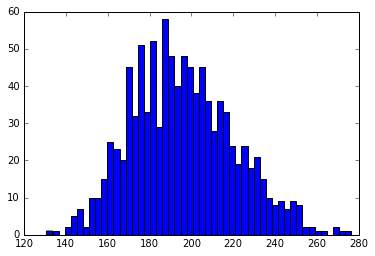
\includegraphics[width=\linewidth]{../../graphs/toy_model_hist_final_prices}
  \caption{Histogram of the final prices for the toy model}
  \label{fig:toymodel}
\end{figure}

\subsection{Parameter estimation}

In order to test our model and code, we test it with real stock prices data.
We selected three companies from NASDAQ-100 index: Baidu, Facebook and Yandex.
The data we used can be found online at Yahoo Finance in CSV format, and in the \texttt{data/historical} folder in our project.
We restricted the data to $300$ days, and calculated the initial stock price, $\mu$ and $\sigma$ from the data in a IPython notebok.
The code is available at \texttt{src/estimate-parameters.ipynb}, and its HTML counterpart can be found at \texttt{docs/noteboks/estimate-parameters.html}.

The estimated parameters are:
\begin{table}[ht]
\centering
\begin{tabular}{|l|l|l|l|}
\hline
Company / Parameter & Initial price & $\sigma$    & $\mu$      \\
\hline
Baidu               & 207.33        & -0.0004196  & 0.02143578 \\
\hline
Facebook            & 83.30         & 0.00135278  & 0.00401862 \\
\hline
Yandex              & 15.45         & -7.9067e-05 & 0.03078405 \\
\hline
\end{tabular}
\end{table}

There parameters were hardcoded into the CUDA simulation at compile time, using the \texttt{Makefile}.

\subsection{CUDA}

The CUDA implementation allowed us to simulate in parallel each path (Markov Chain).
Without parallelization, the usual way to generate the paths would be to simulate a single Markov Chain, and take $M$ samples (one every $n$ steps) after the warmup, assuming that $n$ is large enough to make the sampled paths memoryless.
Thanks to the parallelization, we can simulate $M$ independent paths from the beginning, and after the warmup iterations just take one sample from every independent path.
Not only it is faster but we do not need to make the assumption about the memory we made in the previous implementation.

However, translating the original implementation into CUDA came with some drawbacks due to the nature of the simulation.
First, since we are running the Metropolis algorithm we need to store in each thread the previous path, which is innefficient as memory communication in GPUs is slower than actual computation.
Second, we could not use the standard random number generator as it was too slow and we had no guarantees that every thread generated a pseudo-random number independently. We use the CUDA library for random number generation to solve this.
Finally, the output files were too large to deal with them in the IPython notebook directly.
We solved this by automatically compressing the output and decompressing it in IPython once it has been loaded into the notebook.

All in all, because the extensive amounts of memory needed in every thread to compute the path simulation and the communication overhead this introduces, CUDA was not as fast as expected, but still orders of magnitude faster than the Python toy model implementation.
The complete simulation for one company (640 threads or final paths with 1000 warmup iterations each one, and 3000 time discretization steps in each path) runs in about one minute.

The CUDA source code can be found in \texttt{src/asian-options-main.cu} (main function), \texttt{src/asian-options.cu} (simulation functions) and \texttt{src/asian-options.h} (definitions).

\section{\label{sec:results}Results}

TODO

\section{\label{sec:conclusions}Conclusions}

TODO: What works and what doesnt

% New page
\clearpage

% Bibliography
\bibliography{references}
\bibliographystyle{unsrtnat}

\end{document}
%
% ****** End of file final-report.tex ******
